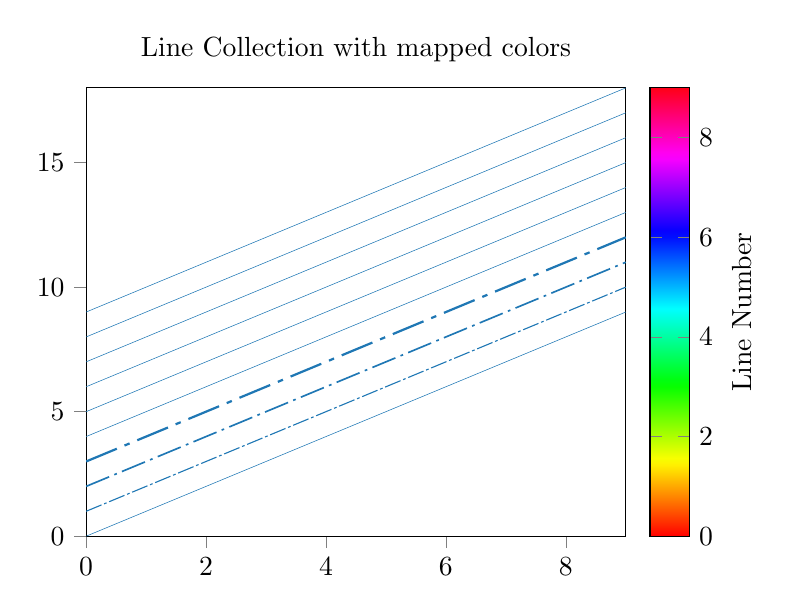
\begin{tikzpicture}

\definecolor{color0}{rgb}{0.12156862745098,0.466666666666667,0.705882352941177}

\begin{axis}[
colorbar,
colorbar style={ylabel={Line Number}},
colormap={mymap}{[1pt]
  rgb(0pt)=(1,0,0);
  rgb(10pt)=(1,0.9375,0);
  rgb(11pt)=(0.96875,1,0);
  rgb(21pt)=(0.03125,1,0);
  rgb(22pt)=(0,1,0.0625);
  rgb(32pt)=(0,1,1);
  rgb(42pt)=(0,0.0625,1);
  rgb(43pt)=(0.03125,0,1);
  rgb(53pt)=(0.96875,0,1);
  rgb(54pt)=(1,0,0.9375);
  rgb(63pt)=(1,0,0.09375)
},
point meta max=9,
point meta min=0,
tick align=outside,
tick pos=left,
title={Line Collection with mapped colors},
x grid style={white!69.01960784313725!black},
xmin=0, xmax=9,
y grid style={white!69.01960784313725!black},
ymin=0, ymax=18
]
\path [draw=color0, very thin, dash pattern=on 3pt off 0pt on 0pt off 0pt]
(axis cs:0,0)
--(axis cs:1,1)
--(axis cs:2,2)
--(axis cs:3,3)
--(axis cs:4,4)
--(axis cs:5,5)
--(axis cs:6,6)
--(axis cs:7,7)
--(axis cs:8,8)
--(axis cs:9,9);

\path [draw=color0, dash pattern=on 6pt off 1pt on 1pt off 1pt]
(axis cs:0,1)
--(axis cs:1,2)
--(axis cs:2,3)
--(axis cs:3,4)
--(axis cs:4,5)
--(axis cs:5,6)
--(axis cs:6,7)
--(axis cs:7,8)
--(axis cs:8,9)
--(axis cs:9,10);

\path [draw=color0, semithick, dash pattern=on 9pt off 2pt on 1pt off 2pt]
(axis cs:0,2)
--(axis cs:1,3)
--(axis cs:2,4)
--(axis cs:3,5)
--(axis cs:4,6)
--(axis cs:5,7)
--(axis cs:6,8)
--(axis cs:7,9)
--(axis cs:8,10)
--(axis cs:9,11);

\path [draw=color0, thick, dash pattern=on 12pt off 3pt on 2pt off 3pt]
(axis cs:0,3)
--(axis cs:1,4)
--(axis cs:2,5)
--(axis cs:3,6)
--(axis cs:4,7)
--(axis cs:5,8)
--(axis cs:6,9)
--(axis cs:7,10)
--(axis cs:8,11)
--(axis cs:9,12);

\path [draw=color0, very thin, dash pattern=on 3pt off 0pt on 0pt off 0pt]
(axis cs:0,4)
--(axis cs:1,5)
--(axis cs:2,6)
--(axis cs:3,7)
--(axis cs:4,8)
--(axis cs:5,9)
--(axis cs:6,10)
--(axis cs:7,11)
--(axis cs:8,12)
--(axis cs:9,13);

\path [draw=color0, very thin, dash pattern=on 3pt off 0pt on 0pt off 0pt]
(axis cs:0,5)
--(axis cs:1,6)
--(axis cs:2,7)
--(axis cs:3,8)
--(axis cs:4,9)
--(axis cs:5,10)
--(axis cs:6,11)
--(axis cs:7,12)
--(axis cs:8,13)
--(axis cs:9,14);

\path [draw=color0, very thin, dash pattern=on 3pt off 0pt on 0pt off 0pt]
(axis cs:0,6)
--(axis cs:1,7)
--(axis cs:2,8)
--(axis cs:3,9)
--(axis cs:4,10)
--(axis cs:5,11)
--(axis cs:6,12)
--(axis cs:7,13)
--(axis cs:8,14)
--(axis cs:9,15);

\path [draw=color0, very thin, dash pattern=on 3pt off 0pt on 0pt off 0pt]
(axis cs:0,7)
--(axis cs:1,8)
--(axis cs:2,9)
--(axis cs:3,10)
--(axis cs:4,11)
--(axis cs:5,12)
--(axis cs:6,13)
--(axis cs:7,14)
--(axis cs:8,15)
--(axis cs:9,16);

\path [draw=color0, very thin, dash pattern=on 3pt off 0pt on 0pt off 0pt]
(axis cs:0,8)
--(axis cs:1,9)
--(axis cs:2,10)
--(axis cs:3,11)
--(axis cs:4,12)
--(axis cs:5,13)
--(axis cs:6,14)
--(axis cs:7,15)
--(axis cs:8,16)
--(axis cs:9,17);

\path [draw=color0, very thin, dash pattern=on 3pt off 0pt on 0pt off 0pt]
(axis cs:0,9)
--(axis cs:1,10)
--(axis cs:2,11)
--(axis cs:3,12)
--(axis cs:4,13)
--(axis cs:5,14)
--(axis cs:6,15)
--(axis cs:7,16)
--(axis cs:8,17)
--(axis cs:9,18);

\end{axis}

\end{tikzpicture}